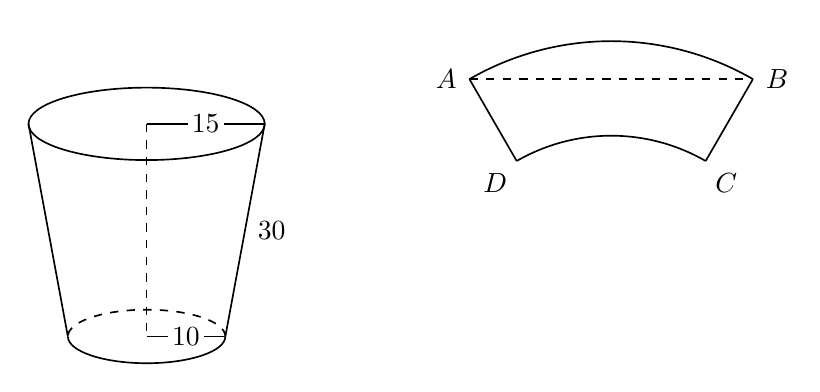
\begin{tikzpicture}[line width=.6pt,font=\normalsize,x=1cm,y=1cm]
% ---- left panel: frustum ----
\coordinate (TC) at (0,2.7);
\coordinate (BC) at (0,0);
\coordinate (Tl) at (-1.5,2.7);
\coordinate (Tr) at (1.5,2.7);
\coordinate (Bl) at (-1,0);
\coordinate (Br) at (1,0);
\coordinate (O) at (5.9,0.15);
\coordinate (A) at (4.1,3.268);
\coordinate (B) at (7.7,3.268);
\coordinate (C) at (7.1,2.228);
\coordinate (D) at (4.7,2.228);
\draw (TC) ellipse [x radius=1.5, y radius=0.46];
\draw (Bl) arc [start angle=180, end angle=360, x radius=1, y radius=0.34];
\draw[dashed] (Br) arc [start angle=0, end angle=180, x radius=1, y radius=0.34];
\draw (Tl) -- (Bl);
\draw (Tr) -- (Br);
\draw[dashed] (TC) -- (BC);
\draw (TC) -- (Tr) node[midway, fill=white, inner sep=1.5pt] {15};
\draw (BC) -- (Br) node[midway, fill=white, inner sep=1.5pt] {10};
\node[anchor=west, inner sep=1.5pt] at (1.35,1.35) {30};
% ---- right panel: unwrapped lateral surface ----
\draw (B) arc [start angle=60, end angle=120, radius=3.6];
\draw (C) arc [start angle=60, end angle=120, radius=2.4];
\draw (A) -- (D);
\draw (B) -- (C);
\draw[dashed] (A) -- (B);
\node[anchor=east, inner sep=1.5pt] at (4,3.268) {$A$};
\node[anchor=west, inner sep=1.5pt] at (7.8,3.268) {$B$};
\node[anchor=north east, inner sep=1.5pt] at (4.64,2.128) {$D$};
\node[anchor=north west, inner sep=1.5pt] at (7.16,2.128) {$C$};
\end{tikzpicture}
